\documentclass[a4paper, 10pt]{article}
\usepackage[margin = 1in]{geometry}
\usepackage{amsmath}
\usepackage{tabularx}
\usepackage{framed}
\setlength{\parindent}{0em}
\newcolumntype{L}{>{\arraybackslash}m{10cm}}
\newcolumntype{T}{>{\arraybackslash}m{6cm}}
\usepackage{graphicx}
\usepackage{pdfpages}

\begin{document}

\section*{Topic 18 - Alternating Currents}
\section{Characteristics of AC}

An alternating current \textbf{varies periodically} with time in magnitude and direction.

\begin{center}
   \begin{tabular}{c | T}
      Term & Definition \\
      \hline
      Period, $T$ & Time taken for one complete cycle \\ 
      \hline
      Frequency, $F$  & Number of complete cycles per unit time \\
      \hline
      Peak current, $I_0$ & Amplitude of current \\
      \hline
   \end{tabular}
\end{center}

\section{Sinusoidal a.c.}
\begin{center}
  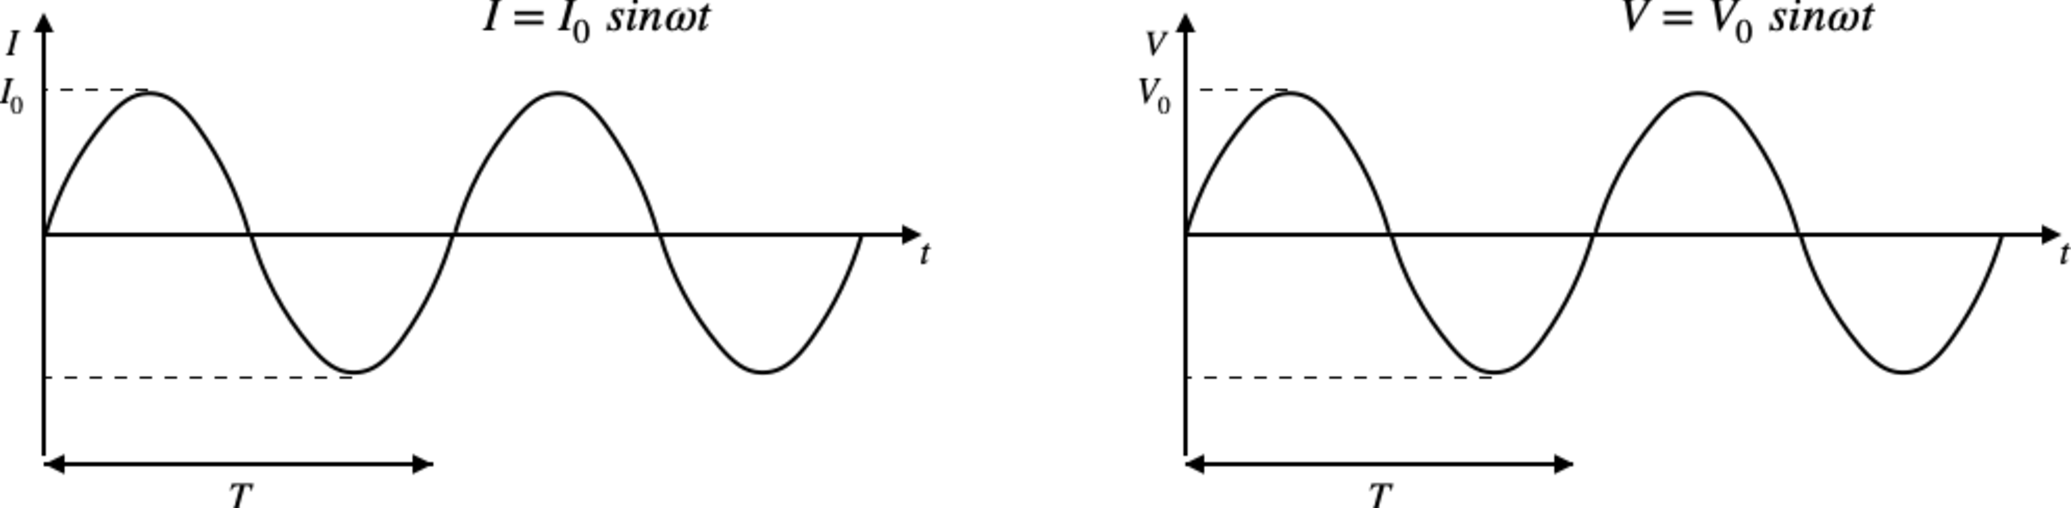
\includegraphics[width=5in]{figures/1.pdf}  
\end{center}	

\section{Power in a.c. circuit}
For a simple resistive circuit with resistor $R$, and an a.c. source,
\[
   V_{ac} = I_{ac} R
\]
\[
   P_{ac} = I_{ac} V_{ac} = I_{ac}^2 R = \frac{V_{ac}^2}{R}
\]
\begin{itemize}
   \item Energy dissipated is the area under the $P_{ac} - t$ graph
   \item Power at any moment is equal to the product of I and V, hence $P$ varies periodically with time,
   \item $P_{min} = 0$ when $I = V =  0$ 
   \item $P_0 = I_0 V_0$ 
\end{itemize}	

\subsection{Mean power, $\langle P_{ac} \rangle$}
\[
   \langle P_{ac} \rangle= \frac{\text{Total energy dissipated in time t}}{t}
\]
\[
   \langle P_{ac} \rangle= \frac{\text{area under $P_{ac} - t$ graph in time $t$ }}{t}
\]

\[
   \langle P_{ac} \rangle = \left( I_{rms} \right)^2 R
\]

\begin{framed}
   The r.m.s. value of an alternating current or voltage is the value of a \textbf{steady} direct current or voltage that would produce thermal energy at the \textbf{same rate} in a given resistor

   \[
      \langle P \rangle = I_{rms}^2 R = \frac{V_{rms}^2}{R} = I_{rms} V_{rms}
   \]
   
\end{framed}	
The rms value can be found by
\begin{enumerate}
   \item Squaring the instantaneous current $I$ 
   \item finding \textbf{mean} value of $I^2$ 
   \item Taking the \textbf{square root} of the mean value
\end{enumerate}	
\[
   I_{rms} = \sqrt{\frac{\int_0^T I^2 dt}{T}} = \sqrt{\langle I^2 \rangle}
\]

\begin{framed}
For a sinusoidal current and voltage 
\[
   I_{rms} = \frac{I_0}{\sqrt{2}}
\]

\[
   V_{rms} = \frac{V_0}{\sqrt{2}}
\]
\[
   \langle P \rangle = I_{rms} V_{rms} = \left( \frac{I_0}{\sqrt{2}} \right) \left( \frac{V_0}{\sqrt{2}} \right)  = \frac{P_0}{2}
\]
\end{framed}	

\section{Transformer}
\begin{center}
   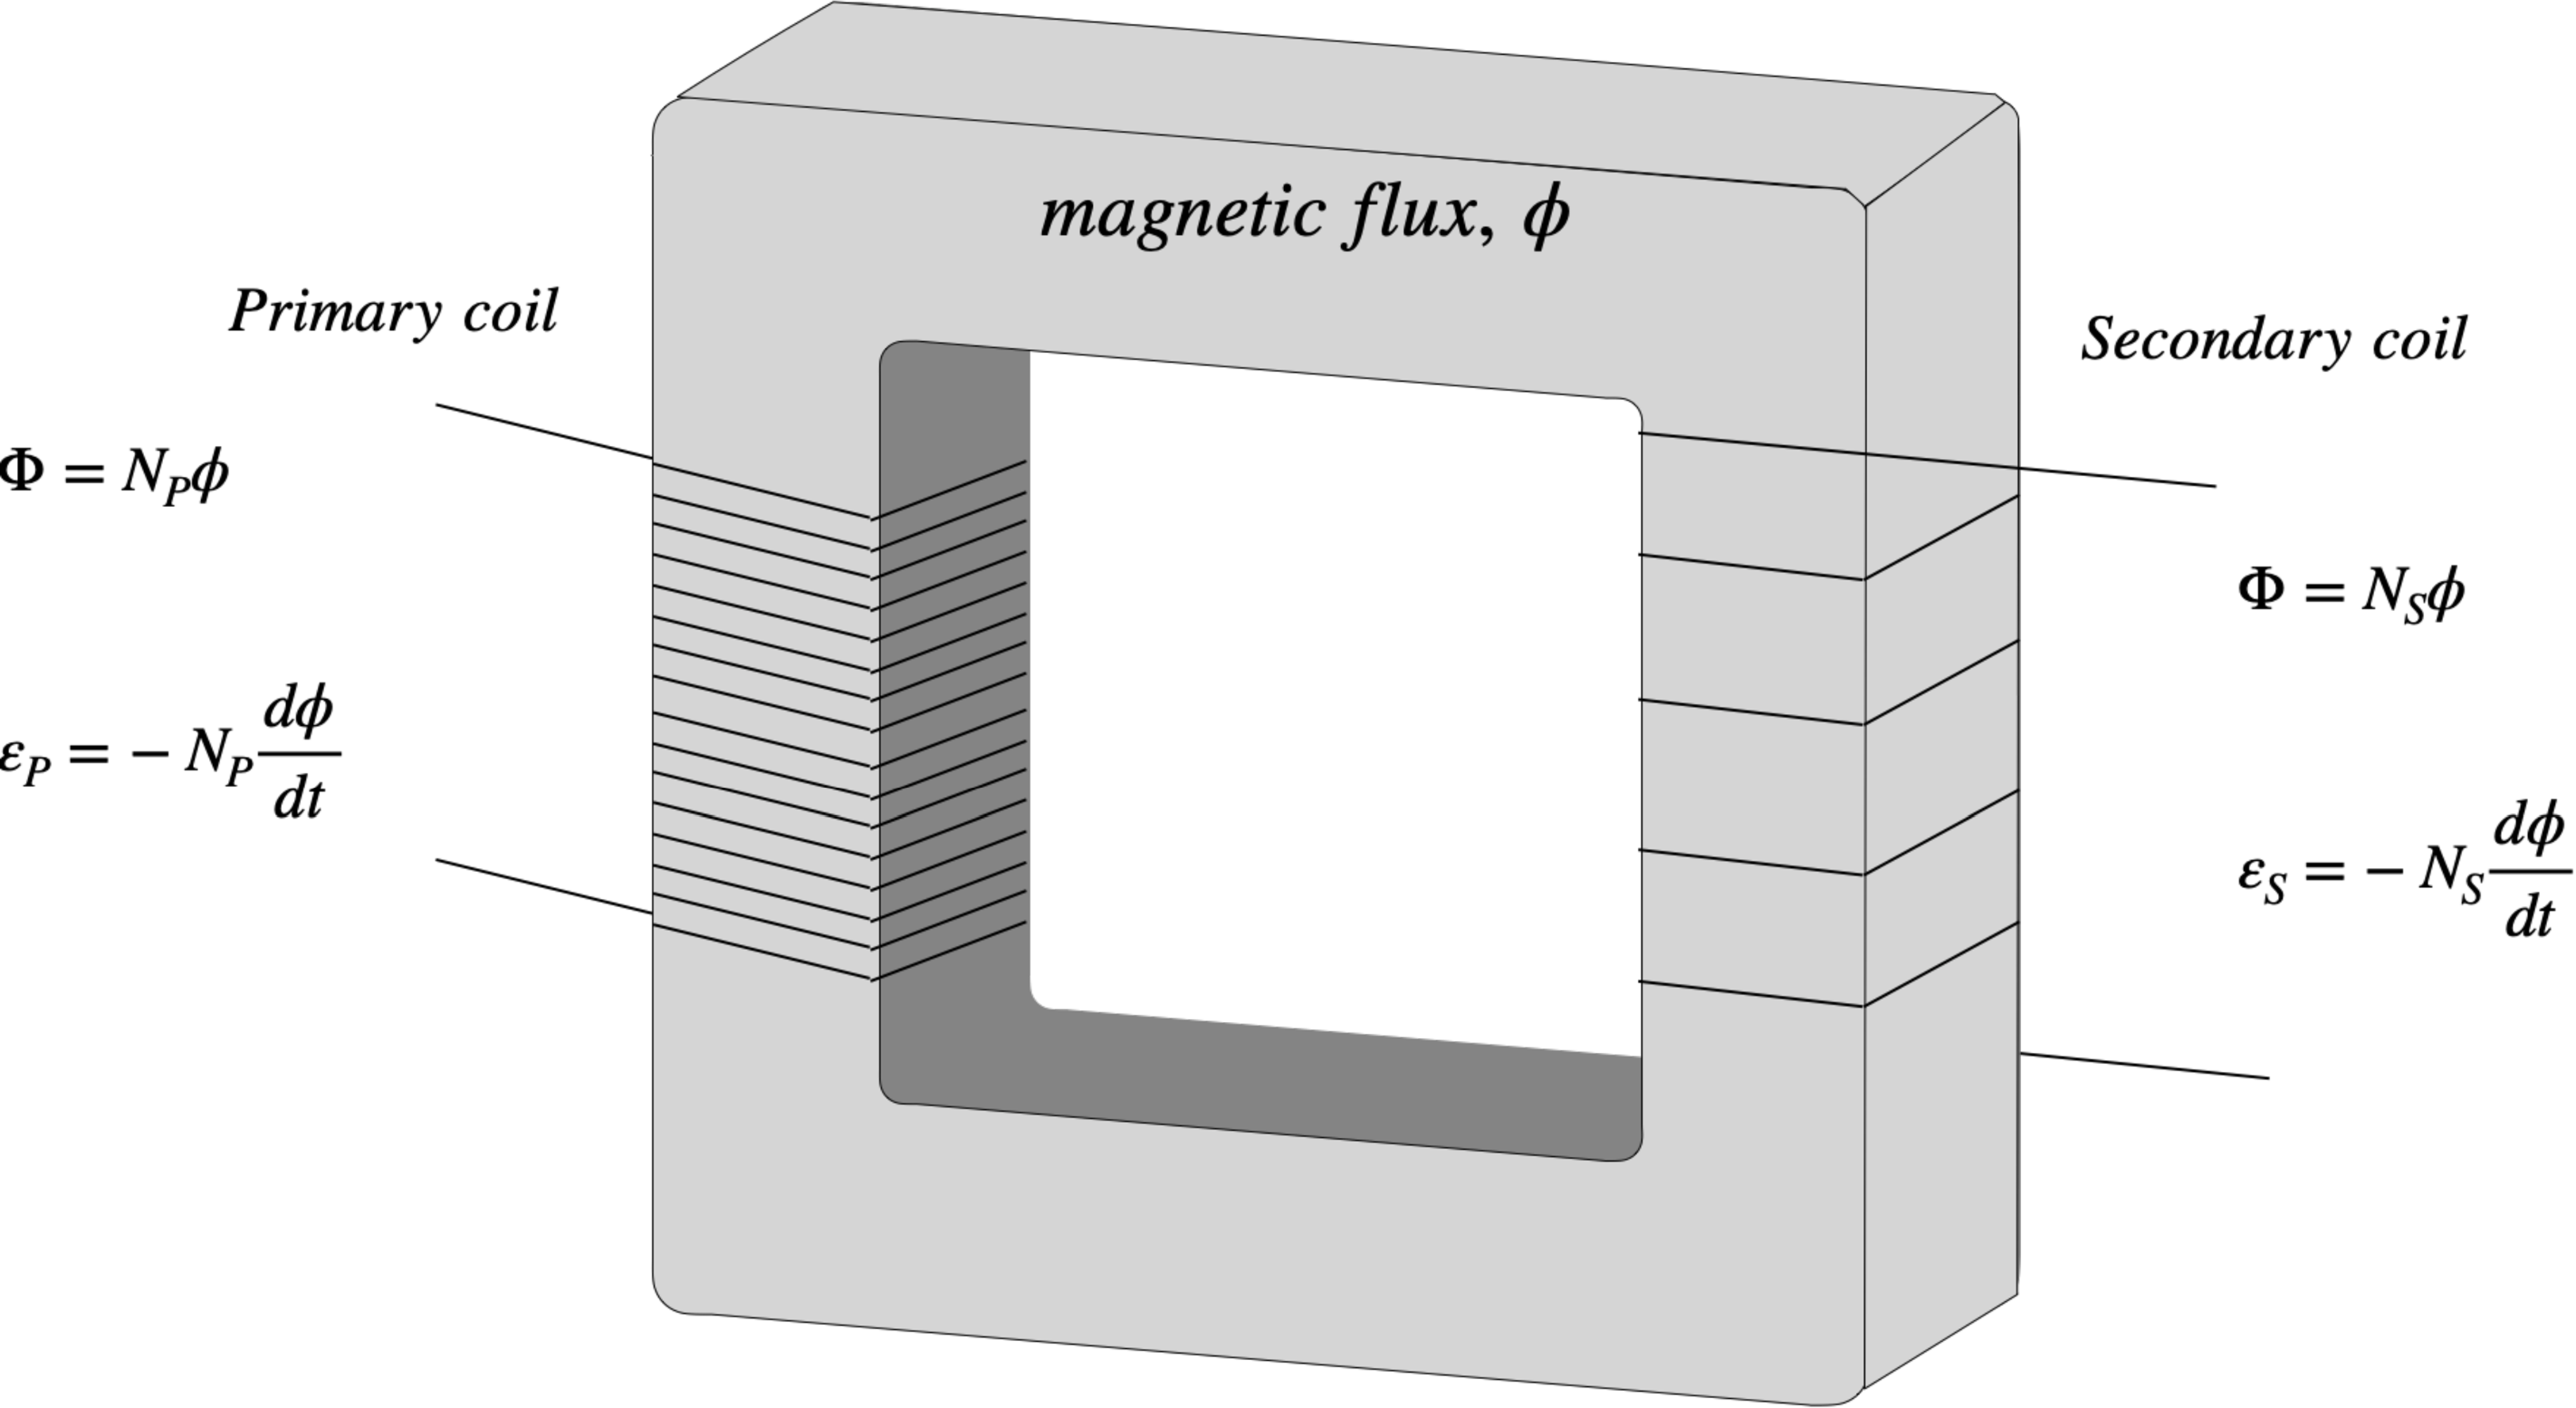
\includegraphics[width=5in]{figures/2.pdf} 
\end{center}	
\begin{itemize}
   \item \textbf{Function}: to use mutual electromagnetic induction to step up or step down voltage
   \item a common iron core is used to concentrate magnetic flux through both coils
   \item AC current flows in primary coil, setting up an alternating magnetic flux in the iron core
   \item According to Faraday's law, the alternating magnetic flux linkage through both coils induces an alternating e.m.f. across each turn in both coils
\end{itemize}	

\subsection{Derivation of results}
since the magnetic flux $\phi$ is the same \textbf{through each turn} for both coils, the induced emf is the same through each turn
\[
\frac{\varepsilon_P}{N_P} = \frac{\varepsilon_S}{N_S} 
\]

\[
\frac{\varepsilon_S}{\varepsilon_P} = \frac{N_S}{N_P}
\] 

Assuming $0$ resistance for an ideal transformer,
\[
\frac{V_S}{V_P} = \frac{\varepsilon_S}{\varepsilon_P} = \frac{N_S}{N_P}
\]

Assuming no power loss for an ideal transformer, input power = output power hence
\[ 
   \frac{I_P}{I_S} = \frac{V_S}{V_P} = \frac{N_S}{N_P}
\]

\subsection{Power loss and design features}
\begin{center}
   \begin{tabular}{T | T}
      Cause of power loss & Design features \\
      \hline
      Joule heating of cooper wires & Thick copper wires of low resistance used \\ \\
      Heating due to \textbf{eddy currents} in iron core & The iron core is made of laminated sheets curring across path of eddy currents, to increase resistance to current flow \\ \\
      Hysteresis loss & Soft iron is used, which can be easily magnetised and demagnetised \\ \\
      Magnetic flux leakage & Iron core maximises flux linkage, E-I shaped iron core is used 
   \end{tabular}
\end{center}

\section{Transmission of electrical power}

For a supply power $P$, transmitting at voltage $V$  and current $I$, and total cable resistance $R$, the power loss is
\[
   P_{loss} = I^2 R = \left( \frac{P}{V} \right)^2 R
\]
\begin{itemize}
   \item hence a high voltage is used to minimise power loss
\end{itemize}	

Alternatively, the power loss can be found by first finding p.d. across cable
\[
   V_{cable} = IR = \left( \frac{P}{V} \right)  R
\]

Power loss is the power dissipated in cable
\[
   P_{loss} = I^2 R = \frac{V_{cable}^2}{R} = \left( \frac{P}{V} \right)^2 R
\]

\section{Rectification with diode}
\begin{center}
   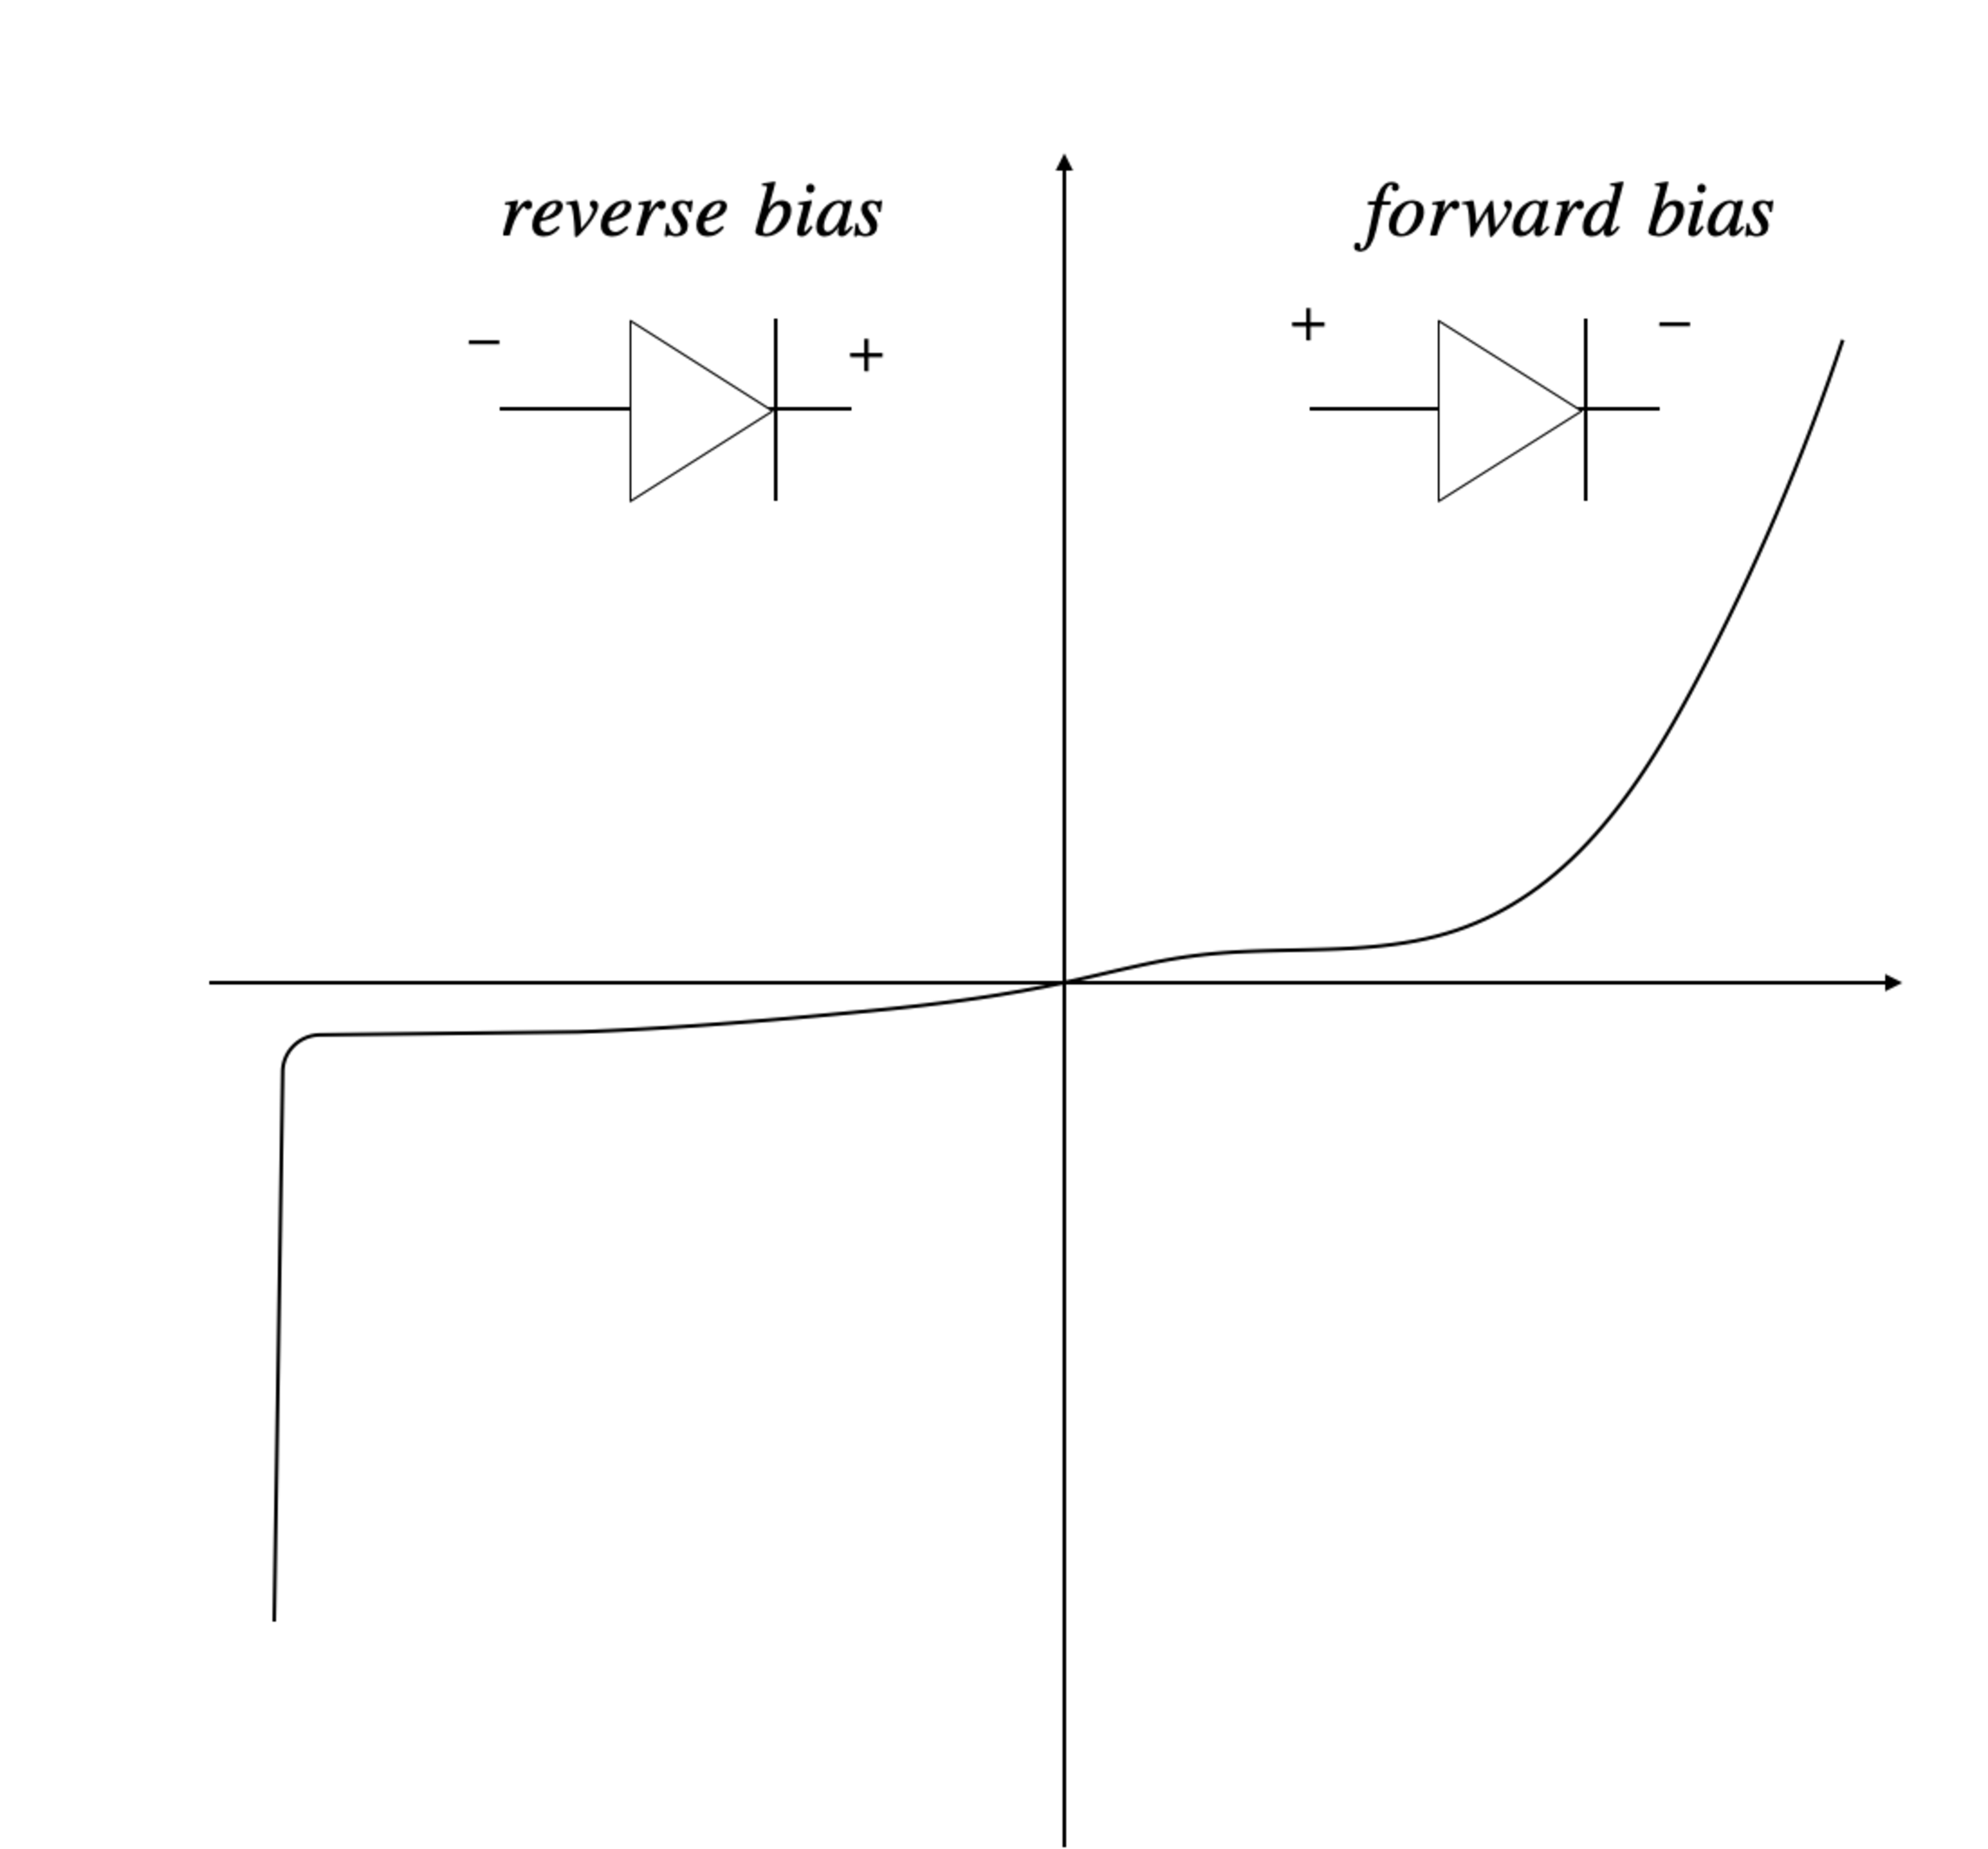
\includegraphics[width=3in]{figures/3.pdf} 
\end{center}	



\end{document}	

